\section{Query Strategy}\label{sec:QueryStrategy}

\autoref{fig:RMBProcessFlow} provides a high-level abstraction of the Resource Management Board. The process flow can be divided into three different views (i.e., \acrshort*{SPARQL}, data processing, and user interface). While the user interface has been outlined in the previous section, data processing will be introduced in the next section. The current section focuses on the \acrshort*{SPARQL} query strategy. When users interact with the \acrshort*{RMB}, the underlying \acrshort*{SPARQL} processes for requesting or updating data are composed automatically, since users are not supposed to form a query by themselves. This section provides the specifications for this \acrshort*{SPARQL} abstraction, specifically focusing on five central stages within the query process, as denoted by the letters {\small \hyperref[ssec:QS-A]{\(\mathcal{A}\)}} to {\small \hyperref[ssec:QS-E]{\(\mathcal{E}\)}} within the \acrshort*{SPARQL} lane in \autoref{fig:RMBProcessFlow}. 

\begin{figure}[H]
	\centering \begin{tikzpicture}
	\node[anchor=south west,inner sep=0] (image) at (0,0,0) {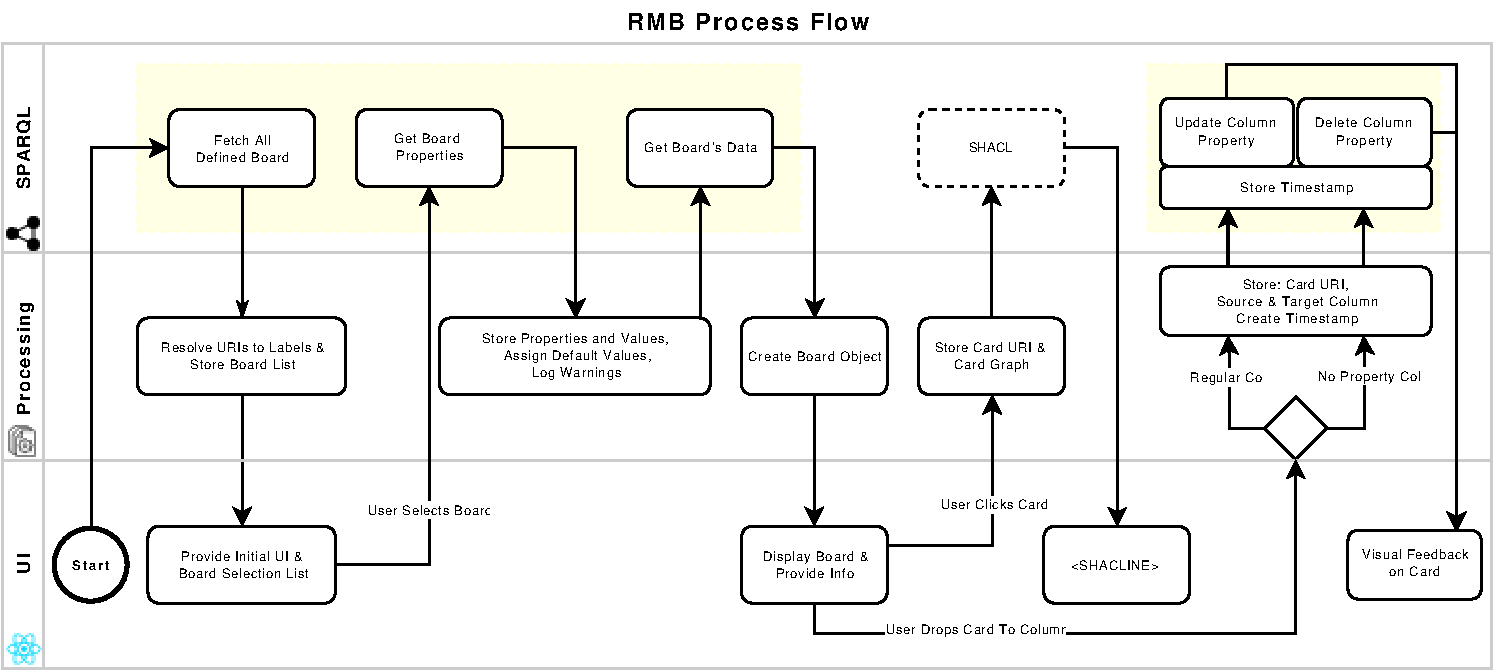
\includegraphics[angle=90,width=83mm]{img/RMB-Flowchart.pdf}};
	\begin{scope}[x={(image.south east)},y={(image.north west)}]

	\draw (0.105,0.160) node[anchor=west] {\rotatebox{90}{\small \hyperref[ssec:QS-A]{\(\mathcal{A}\)}}};
	\draw (0.105,0.290) node[anchor=west] {\rotatebox{90}{\small \hyperref[ssec:QS-B]{\(\mathcal{B}\)}}};
	\draw (0.105,0.465) node[anchor=west] {\rotatebox{90}{\small \hyperref[ssec:QS-C]{\(\mathcal{C}\)}}};
	\draw (0.090,0.805) node[anchor=west] {\rotatebox{90}{\small \hyperref[ssec:QS-D]{\(\mathcal{D}\)}}};
	\draw (0.090,0.915) node[anchor=west] {\rotatebox{90}{\small \hyperref[ssec:QS-E]{\(\mathcal{E}\)}}};
	
	\end{scope}
	\end{tikzpicture}
	\caption[Process Flow of the \tracknshrink{RMB}]{Process flow of the \acrshort*{RMB} separated by three views (i.e., \acrshort*{SPARQL}, data processing, and \acrshort*{UI}).}
	\label{fig:RMBProcessFlow}
\end{figure}

\noindent All queries will use two interfaces developed by eccenca; Foremost, the \textit{\tracknshrink{SPARQL} logic store} (or sparqlChannel in the following), which requires an input string that contains the actual \acrshort*{SPARQL} query, and returns a response object. The response object may be set to \texttt{responseJson} to receive a \acrshort*{JSON} structure as the output format. The second interface is the \textit{TitleHelper logic store} (or titleHelper in the following) which---in its default configuration---requires a single resource (or an array of resources) as an input argument, and returns a key-value object, whereas a key is an \acrshort*{IRI} and value is the corresponding label.

The following three subsections represent the query stages (i.e., {\small \hyperref[ssec:QS-A]{\(\mathcal{A}\)}}, {\small \hyperref[ssec:QS-B]{\(\mathcal{B}\)}}, and {\small \hyperref[ssec:QS-C]{\(\mathcal{C}\)}}) in order to receive and send the required data for rendering the board.



\subsection[A — Fetch All Defined Boards]{\(\mathcal{A}\) — Fetch All Defined Boards}\label{ssec:QS-A}

Initially, the prototype should send an asynchronous request to fetch all available boards (i.e., board configurations). \autoref{lst:SPARQLFetchAllBoards} illustrates this query, which essentially requesting resources that are of the type \acrshort{rmb}\texttt{BoardConfig} (line 3), as earlier specified in the model for the board configuration. Line 4 requests the board’s description if defined.


\begin{spacing}{0.9}
    \lstset{language=SPARQL,escapechar=|}
    \begin{lstlisting}[
    label={lst:SPARQLFetchAllBoards},
    xleftmargin=8em, % this needs to be manually adjusted to center the frame
    xrightmargin=-8em, % this needs to be manually adjusted to center the frame
    caption={[A — \tracknshrink{SPARQL} Request To Fetch All Boards]Requesting all boards that are of type \acrshort{rmb}\texttt{BoardConfig}.}]
SELECT DISTINCT ?board ?descr
WHERE {
  ?board a <|\url{https://vocab.eccenca.com/rmb/BoardConfig}|> .
  OPTIONAL { ?board <|\url{http://purl.org/dc/terms/description}|> ?descr . }
}
\end{lstlisting}
\end{spacing}

\noindent \autoref{lst:JSONFetchAllBoards} illustrates the response object that contains the board configuration of the first use case, as earlier defined in \autoref{lst:FOAFBoardConfig}. The \textit{titleHelper} would reveal the title as also defined in former board configuration (i.e., \acrshort*{FOAF} Term Status). Nevertheless, the list of board titles should be used in the \texttt{<SelectBox>} element, which was shown previously in \autoref{fig:BoardTemplateMDL} (1).

\begin{spacing}{0.9}
    \lstset{language=JavaScript}
    \begin{lstlisting}[
    label={lst:JSONFetchAllBoards},
    xleftmargin=2.5em, % this needs to be manually adjusted to center the frame
    xrightmargin=-2.5em, % this needs to be manually adjusted to center the frame
    caption={[A — Response Object]Exemplary response object of the request in \autoref{lst:SPARQLFetchAllBoards}.}]
[{
  "board": {"type":"uri",    "value":"https://vocab.eccenca.com/rmb/foaf-term-status"},
  "descr": {"type":"literal","value":"Manages terms by their status in the FOAF namespace"}
},{ 
  // other configurations
}]
\end{lstlisting}
\end{spacing}

\vspace*{-1.55em}


\subsection[B — Get Board Properties]{\(\mathcal{B}\) — Get Board Properties}\label{ssec:QS-B}


Selecting a board from the \texttt{<SelectBox>} immediately triggers another query requesting all properties within the selected board configuration. That is, the properties and their values as requested in the first functional requirement \tracknshrink{FR}\textsubscript{1} or similar in \autoref{tab:BoardConfig}. This query, however, requires the \acrshort*{IRI} of the board the user selected. \autoref{lst:SPARQLGetBoardProperties} illustrates the  request for all properties and values of a specific board, using the placeholder variable \texttt{boardIRI} in line 3.


\begin{spacing}{0.9}
    \lstset{language=SPARQL,escapechar=|}
    \begin{lstlisting}[
    label={lst:SPARQLGetBoardProperties},
    xleftmargin=20em, % this needs to be manually adjusted to center the frame
    xrightmargin=-20em, % this needs to be manually adjusted to center the frame
    caption={[B — \tracknshrink{SPARQL} Request To Fetch Board Properties]Requesting all defined properties of a specific board (i.e., the variable \texttt{boardIRI}).}]
SELECT DISTINCT ?p ?o
WHERE {
  <boardIRI> ?p ?o .
}
\end{lstlisting}
\end{spacing}

\noindent Consider the scenario that the current board configuration contains the information of the first use case, as illustrated in \autoref{lst:FOAFBoardConfig} or \autoref{fig:BoardConfigs} (B), and the former request replaces the placeholder \texttt{boardIRI} with \acrshort{rmb}\texttt{foaf-term-status} (\autoref{lst:SPARQLGetBoardProperties} line 3). As a result, the sparqlChannel would return a response object similar as depicted by \autoref{lst:JSONGetBoardProperties}.

This output provides two important information: (1) the developer knows what specific properties have been defined within the selected board configuration (i.e., lines containing \texttt{"p")}, and (2) what their corresponding object value is (i.e., lines containing \texttt{"o"}). In any case, the response object should match the board configuration regarding their contents, as can be seen in \autoref{lst:JSONGetBoardProperties} and \autoref{fig:BoardConfigs}~(B).



\begin{spacing}{0.9}
    \lstset{language=JavaScript,escapechar=|}
    \begin{lstlisting}[
    label={lst:JSONGetBoardProperties},
    xleftmargin=2.5em, % this needs to be manually adjusted to center the frame
    xrightmargin=-2.5em, % this needs to be manually adjusted to center the frame
    caption={[B — Response Object]Exemplary response object of the request in \autoref{lst:SPARQLGetBoardProperties}. The response matches the board configuration in the \textit{DataManger}. In this instance, the response object matches the config of \autoref{fig:BoardConfigs} (B).}]
[{
  "p": {"type": "uri",    "value": "http://www.w3.org/1999/02/22-rdf-syntax-ns|\textcolor{colString}{\#}|type"},
  "o": {"type": "uri",    "value": "https://vocab.eccenca.com/rmb/BoardConfig"}
},{
  "p": {"type": "uri",    "value": "http://www.w3.org/2000/01/rdf-schema|\textcolor{colString}{\#}|label"},
  "o": {"type": "literal","value": "FOAF Term Status"}
},{
  "p": {"type": "uri",    "value": "http://purl.org/dc/terms/description"},
  "o": {"type": "literal","value": "Manages terms by their status in the FOAF namespace"}
},{
  "p": {"type": "uri",    "value": "https://vocab.eccenca.com/rmb/cardsGraph"},
  "o": {"type": "uri",    "value": "http://xmlns.com/foaf/0.1/"}
},{
  "p": {"type": "uri",    "value": "https://vocab.eccenca.com/rmb/cardsClass"},
  "o": {"type": "uri",    "value": "http://www.w3.org/2002/07/owl|\textcolor{colString}{\#}|Class"}
},{
  "p": {"type": "uri",    "value": "https://vocab.eccenca.com/rmb/cardsClass"},
  "o": {"type": "uri",    "value": "http://www.w3.org/2002/07/owl|\textcolor{colString}{\#}|DatatypeProperty"}
},{
  "p": {"type": "uri",    "value": "https://vocab.eccenca.com/rmb/cardsClass"},
  "o": {"type": "uri",    "value": "http://www.w3.org/2002/07/owl|\textcolor{colString}{\#}|ObjectProperty"}
},{
  "p": {"type": "uri",    "value": "https://vocab.eccenca.com/rmb/cardsColumnProperty"},
  "o": {"type": "uri",    "value": "http://www.w3.org/2003/06/sw-vocab-status/ns|\textcolor{colString}{\#term\_status}|"}
},{
  "p": {"type": "uri",    "value": "https://vocab.eccenca.com/rmb/cardsLaneProperty"},
  "o": {"type": "uri",    "value": "http://www.w3.org/1999/02/22-rdf-syntax-ns|\textcolor{colString}{\#}|type"}
},{
  "p": {"type": "uri",    "value": "https://vocab.eccenca.com/rmb/cardsDescriptionProperty"},
  "o": {"type": "uri",    "value": "http://www.w3.org/2000/01/rdf-schema|\textcolor{colString}{\#}|comment"}
}]
\end{lstlisting}
\end{spacing}


\noindent At this stage, developers can check the existence of all properties and may add default values for missing properties, as specified in \autoref{tab:BoardConfig}. For example, \autoref{lst:JSONGetBoardProperties} does not contain a \texttt{boardLimit} property. However, as outlined in \tracknshrink{FR}\textsubscript{2} (Default Values), it is beneficial to set a limit implicitly, since this will avoid loading too many cards on the board which would likely causes the browser to stall. A default limit of 100 can be considered as a reasonable maximum amount of cards. If this is not high enough, users may set an explicit board limit in the board configuration to override the default value. Lastly, the modified property was not part of the response object. However, since the modified property is used to store a timestamp in the event of dropping a card to a column, it is always justifiable to use an implicit modified property in case the response object lacks its definition. The property   \acrshort{dct}\texttt{modified} is a suitable candidate for this task.

At this stage, it should also be checked if the board contains all the required elements in order to render the board. As indicated in \tracknshrink{FR}\textsubscript{1} and \autoref{tab:BoardConfig}, the response object should contain at least a name, the underlying card’s graph, the card classes, and the column property. If anything is missing, the user should receive a warning provided in the \texttt{<InfoBox>} element, as shown in \autoref{fig:BoardTemplateMDL} (4).




\subsection[C — Get Board’s Data]{\(\mathcal{C}\) — Get Board’s Data}\label{ssec:QS-C}

The last stage is requesting the actual cards that are displayed within the board, along with their requested properties. \autoref{lst:SPARQLGetBoardsData} provides a generic template specification to request this data. In the stage of data processing, the placeholder variables (depicted in red) need to be replaced with the corresponding resources of the former response object (i.e., \autoref{lst:JSONGetBoardProperties}). However, in the case of absent resources, the entire placeholder line within the where clause and the specific placeholder within the projection variables (lines 1 and 2) should be removed in order to form clean query.

The keyword \texttt{SAMPLE} (lines 1 and 2) is an aggregate function that returns an arbitrary value from a multiset passed to it. For example, if there are multiple column values (e.g., \textit{stable} and \textit{unstable}), an arbitrary single selection gets returned.\footnote{Thus, the variable names are mapped from plural to a singular form.} Although this event is likely an indication for broken or invalid data, it should be guaranteed that the response only contains atomic values.\footnote{This operation is similar to the process of achieving a \textit{first normal form} (\libertineLF1\tracknshrink{NF}\libertineOsF) in the field of database normalization. In other words, a table only consists of atomic columns, which means all cells have a single value.}

At first glance, using the keyword \texttt{OPTIONAL} for the \texttt{cardsColumnProperty} (line 7) may seem like an error; however, the optional clause is used on purpose, since only the board configuration requires the definition of that property. For a resource, on the other hand, it is not a necessity to contain the requested property. An example of this scenario is provided in the second use in this work (see page \pageref{fig:RMB Use Case 2}). In this example, the column property (i.e., \acrshort{vs}\texttt{term\_status)} was defined. However, the \tracknshrink{UNESCO} terms did not contain this property, as the purpose of this scenario was to assign it from scratch. Therefore, the \textit{no property} column was listed as a functional requirement in \tracknshrink{FR}\textsubscript{8}. Note that this also applies to the \texttt{cardsLaneProperty} (line 8), as resources will fallback in the \textit{Everything Else} swimlane (see \tracknshrink{FR}\textsubscript{10}).


\begin{spacing}{0.9}
    \lstset{language=SPARQL,escapechar=|}
    \begin{lstlisting}[
    label={lst:SPARQLGetBoardsData},
    xleftmargin=2.2em, % this needs to be manually adjusted to center the frame
    xrightmargin=-2.2em, % this needs to be manually adjusted to center the frame
    caption={[C — \tracknshrink{SPARQL} Template to Request the Board’s Data]Template specification for requesting the content of the board depending on the selected board and card component resources. Variables that need to be replaced or removed are depicted in red color.}]
SELECT DISTINCT ?card (SAMPLE(?columns) AS ?column){laneSample}
  (SAMPLE(?descriptions) AS ?description)(SAMPLE(?modifieds) AS ?modified){additionalValues}
FROM <cardGraph>
WHERE {
  ?card a ?class.
  FILTER (?class IN (<cardsClass>)) .
  OPTIONAL { ?card <cardsColumnProperty> ?columns. }
  OPTIONAL { ?card <cardsLaneProperty> ?lanes. }
  OPTIONAL { ?card <cardsDescriptionProperty> ?descriptions. }
  OPTIONAL { ?card <cardsModifiedProperty> ?modifieds. }
  {additionalPropertiesPlaceholder}
}
GROUP BY ?card
LIMIT boardLimit
\end{lstlisting}
\end{spacing}


\noindent For illustration purposes, \autoref{lst:SPARQLGetBoardsDataDemo} demonstrates the final query after the replacement process of the former \acrshort*{SPARQL} template. As stated, the resources used in \autoref{lst:SPARQLGetBoardsDataDemo} stem from the prior response object of stage {\small \hyperref[ssec:QS-B]{\(\mathcal{B}\)}} (see \autoref{lst:JSONGetBoardProperties}). Moreover, the placeholders for additional properties were removed, since they were not defined in the response object.

\begin{spacing}{0.9}
    \lstset{language=SPARQL,escapechar=|}
    \begin{lstlisting}[
    label={lst:SPARQLGetBoardsDataDemo},
    xleftmargin=2.2em, % this needs to be manually adjusted to center the frame
    xrightmargin=-2.2em, % this needs to be manually adjusted to center the frame
    caption={[C — \tracknshrink{SPARQL} Sample for the First Use Case]\tracknshrink{SPARQL} sample to retrieve the board’s data of the first use case.}]
SELECT DISTINCT ?card (SAMPLE(?columns) AS ?column)(SAMPLE(?lanes) AS ?lane)
  (SAMPLE(?descriptions) AS ?description)(SAMPLE(?modifieds) AS ?modified)
FROM <http://xmlns.com/foaf/0.1/>
WHERE
{
  ?card a ?class.
  FILTER (?class IN (
    <http://www.w3.org/2002/07/owl#Class>,
    <http://www.w3.org/2002/07/owl#DatatypeProperty>,
    <http://www.w3.org/2002/07/owl#ObjectProperty>
  )) .
  OPTIONAL { ?card <http://www.w3.org/2003/06/sw-vocab-status/ns#term_status> ?columns. }
  OPTIONAL { ?card <http://www.w3.org/1999/02/22-rdf-syntax-ns#type> ?lanes. }
  OPTIONAL { ?card <http://www.w3.org/2000/01/rdf-schema#comment> ?descriptions. }
  OPTIONAL { ?card <http://purl.org/dc/terms/modified> ?modifieds. }
}
GROUP BY ?card
LIMIT 100
\end{lstlisting}
\end{spacing}


\noindent \autoref{lst:SPARQLGetBoardsDataDemo} returns a response object that contains all 75 \acrshort*{FOAF} terms.\footnote{To replicate this scenario, you may visit \url{http://bit.ly/foaf-term-status}, which is linking to the \tracknshrink{LOV SPARQL} endpoint containing the query provided in \autoref{lst:SPARQLGetBoardsDataDemo}. The output can be toggled between a raw response (i.e., similar to \autoref{lst:JSONGetBoardsData}), and a table view.} \autoref{lst:JSONGetBoardsData} shows an excerpt of four resources, which are—regarding their content—similar to the mockup provided on page \pageref{fig:RMB Use Case 1}. Ultimately, this array of resources represents the cards of the Resource Management Board.

The \autoref{ssec:DataTransformation} (Data Transformation) will highlight important aspects when converting the final response object (i.e., \autoref{lst:JSONGetBoardsData}) into the prior defined target data model (i.e., \autoref{lst:react-trello-multipleLanesJSON}) in order to satisfy the required format of react-trello.


\begin{spacing}{0.9}
    \lstset{language=JavaScript,escapechar=|}
    \begin{lstlisting}[
    label={lst:JSONGetBoardsData},
    xleftmargin=2.2em, % this needs to be manually adjusted to center the frame
    xrightmargin=-2.2em, % this needs to be manually adjusted to center the frame
    caption={[C — Response Object]Sample response object of the request in \autoref{lst:SPARQLGetBoardsDataDemo}. The object contains four resources (i.e., cards) similar to the mockup of the first use case (see page \pageref{fig:RMB Use Case 1}).}]
[{
    "card":       {"type":"uri",    "value":"http://xmlns.com/foaf/0.1/Document"},
    "column":     {"type":"literal","value":"stable"},
    "lane":       {"type":"uri",    "value":"http://www.w3.org/2002/07/owl#Class"},
    "description":{"type":"literal","value":"A document."},
    "modified":   {"type":"literal","value":"2019-09-06T09:24:37+02:00",
                                    "datatype": "http://www.w3.org/2001/XMLSchema#dateTime"}
  },{
    "card":       {"type":"uri",    "value":"http://xmlns.com/foaf/0.1/mbox"},
    "column":     {"type":"literal","value":"stable"},
    "lane":       {"type":"uri",    "value":"http://www.w3.org/2002/07/owl#ObjectPropert"},
    "description":{"type":"literal","value":"A personal mailbox, ie. an Internet mailbox..."}
  },{
    "card":       {"type":"uri",    "value":"http://xmlns.com/foaf/0.1/depiction"},
    "column":     {"type":"literal","value":"testing"},
    "lane":       {"type":"uri",    "value":"http://www.w3.org/1999/02/22-rdf-syntax-ns#Property"},
    "description":{"type":"literal","value":"A depiction of some thing."}
  },{
    "card":       {"type":"uri",    "value":"http://xmlns.com/foaf/0.1/knows"},
    "column":     {"type":"literal","value":"stable"},
    "lane":       {"type":"uri",    "value":"http://www.w3.org/1999/02/22-rdf-syntax-ns#Property"},
    "description":{"type":"literal","value":"A person known by this person (indicating..."}
}]
\end{lstlisting}
\end{spacing}



\subsection*{Update \& Delete Column Properties}

\noindent The following two subsections will provide the query specifications for column updates. Specifically, an event listener should trigger the process of a column update, whenever a card gets dropped to column. An informal algorithm that handles column updates would be:


\textsf{\small
\begin{addmargin}[1.70em]{1.70em}
(1) When dropping a card, check if the source column \tracknshrink{AND} the target column is equal; then do nothing. (2) If the source column \tracknshrink{AND} target column are unequal, then check
\begin{addmargin}[1.80em]{1.80em}(2A) if the target column equals a column value other than \textit{no property}; then do update the resource’s column property to the target column value (i.e., stage {\small \hyperref[ssec:QS-D]{\(\mathcal{D}\)}}). If (2A) is not the case, check
\end{addmargin}
\begin{addmargin}[1.80em]{1.80em}(2B) if the target column equals the column value of \textit{no property}; then do delete the resource’s column property entirely (i.e., stage {\small \hyperref[ssec:QS-E]{\(\mathcal{E}\)}}).
\end{addmargin}
\end{addmargin}
}
\vspace*{\baselineskip{}}

\subsubsection*{Set a Timestamp}

\noindent Regardless of updating or deleting a property, both stages have in common that they store a timestamp in their process, as can be seen in \autoref{fig:RMBProcessFlow}. Therefore, \autoref{lst:SPARQLTimestamp} specifies a timestamp template that is applicable in both stages. There are two steps involved for updating the value of the modified property: (1) deleting all existing values and (2) inserting the new value. Moreover, the depicted \texttt{DELETE/WHERE} approach (line 1 and 2) guarantees to delete a set of variables.\footnote{See \acrshort*{SPARQL} specification: \url{https://www.w3.org/TR/sparql11-update/\#deleteInsert}.} This essentially means that if there are multiple timestamps values, the query will delete all of them.\footnote{Although this should not occur though, due to sampling the projection variables beforehand (see \autoref{lst:SPARQLGetBoardsData}).} Similar to the prior templates, placeholder variables are depicted in red color. In order to update a value the query needs to know (in descending order): the resource’s graph (i.e., \texttt{cardsGraph}), its resource identifier (i.e., \texttt{cardId}), and the property that needs to be adjusted (i.e., \texttt{cardsModifiedProperty}). The timestamp is provided in \tracknshrink{ISO} 8601.\footnote{The \tracknshrink{ISO} 8601 is a standardized time format, which has the following pattern: \libertineLF2019-12-20T08:30:00+01:00\libertineOsF. That is expressing the date of December 20, 2019, at a time of 8:30:00, and a one hour time offsets from \tracknshrink{UTC}.}


\begin{spacing}{0.9}
    \lstset{language=SPARQL,escapechar=|}
    \begin{lstlisting}[
    label={lst:SPARQLTimestamp},
    xleftmargin=11em, % this needs to be manually adjusted to center the frame
    xrightmargin=-11em, % this needs to be manually adjusted to center the frame
    caption={[\tracknshrink{SPARQL} Template to Update the Modified Property]\tracknshrink{SPARQL} template to update the modified property of a resource.}]
WITH <cardsGraph>
DELETE { <cardId> <cardsModifiedProperty> ?o . }
WHERE  { <cardId> <cardsModifiedProperty> ?o } ;
  INSERT DATA {
    GRAPH <cardsGraph> {
      <cardId>
      <cardsModifiedProperty>
      "ISO8601Timestamp"^^<http://www.w3.org/2001/XMLSchema#dateTime> .
    }
  }
\end{lstlisting}
\end{spacing}


% \vspace*{-1.20em}

\newpage

\subsection[D — Update Column Property]{\(\mathcal{D}\) — Update Column Property}\label{ssec:QS-D}

The query for updating a timestamp has a similar pattern as the query for updating a column property. This means that all instances of \texttt{cardsModifiedProperty} will be replaced by \texttt{cardsColumnProperty}. However, in the stage of data processing, the resource for \texttt{newColumnValue} (line 8) should be type-checked, since it may either be an \acrshort*{IRI} or a literal. Hence, it is either surrounded by angle brackets (\texttt{<>}) or double quotes (\texttt{""}), respectively.


\begin{spacing}{0.9}
    \lstset{language=SPARQL,escapechar=|}
    \begin{lstlisting}[
    label={lst:SPARQLColumnUpdate},
    xleftmargin=11em, % this needs to be manually adjusted to center the frame
    xrightmargin=-11em, % this needs to be manually adjusted to center the frame
    caption={[D — \tracknshrink{SPARQL} Template to Update the Column Property]\tracknshrink{SPARQL} template to update the column property of a resource.}]
WITH <cardsGraph>
DELETE { <cardId> <cardsColumnProperty> ?o . }
WHERE  { <cardId> <cardsColumnProperty> ?o } ;
  INSERT DATA {
    GRAPH <cardsGraph> {
      <cardId>
      <cardsColumnProperty>
      <"newColumnValue"> .
    }
  }
\end{lstlisting}
\end{spacing}


\vspace*{-1.20em}


\subsection[E — Delete Column Property]{\(\mathcal{E}\) — Delete Column Property}\label{ssec:QS-E}

If a user drags a card to the \textit{no property} column, the corresponding column property of that resource gets deleted using \autoref{lst:SPARQLColumnDelete}.

\begin{spacing}{0.9}
    \lstset{language=SPARQL,escapechar=|}
    \begin{lstlisting}[
    label={lst:SPARQLColumnDelete},
    xleftmargin=11em, % this needs to be manually adjusted to center the frame
    xrightmargin=-11em, % this needs to be manually adjusted to center the frame
    caption={[E — \tracknshrink{SPARQL} Template to Delete the Column Property]\tracknshrink{SPARQL} template to delete the column property of a resource.}]
WITH <cardsGraph>
DELETE { <cardId> <cardsColumnProperty> ?o . }
WHERE  { <cardId> <cardsColumnProperty> ?o } ;
\end{lstlisting}
\end{spacing}

\vspace*{-1.20em}